\documentclass{beamer}

\usepackage[utf8]{inputenc}
\usepackage{default}
\usepackage{pslatex}
\usepackage{graphicx}
% \usepackage{algorithmic}
\usepackage{multicol}
\usepackage[french]{babel}

\usetheme{Warsaw}

\title{Comment simuler numériquement la géomorphologie alpine ?}
\subtitle{Sujet de TPE}
\author{Gros Alexis, Manceau Thibaut, Porteries Tristan}
% \logo{
\includegraphics[height=0.5cm]{blender.png}}

\makeindex

\useoutertheme{infolines}

\begin{document}

% Titre
\frame{\titlepage}

% Sommaire
\begin{frame}{Sommaire}
\small \tableofcontents
\end{frame}

\section{Les phénomènes géormophologiques}
\subsection{La subduction}
\begin{frame}
\end{frame}

\subsection{L'obduction}
\begin{frame}
\end{frame}

\section{L'érosion}
\subsection{L'altération mécanique}
\begin{frame}
\end{frame}

\subsection{L'altération physico-chimique}
\begin{frame}
\end{frame}

\section{Le système cellulaire}
\subsection{Les cellules}
\begin{frame}
  Cellule : le plus petit élément de la simulation incompressible, représenté par une sphère de diamètre 1. \smallbreak
  Propriétés mutables :
  \begin{itemize}
   \item vélocité ;
   \item position ;
   \item cellules adjacentes.
  \end{itemize}
  Propriétés immuables :
  \begin{itemize}
   \item plaque tectonique.
  \end{itemize}
  Disposition en nid-d'abeille au lancement de la simulation.
  \begin{center}
    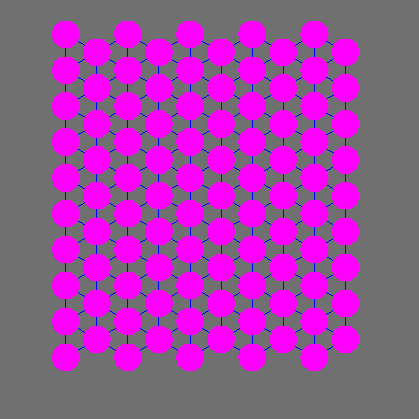
\includegraphics[width=4cm]{Images/hexagone.png}
  \end{center}
\end{frame}

\subsection{La propagation par fronts}
\begin{frame}
  Propagation par front, l’ancien front créer le nouveau. Le premier front ne contient que la cellule en collision.
  Chaque cellule du front interagissent avec les cellules après le front.
  \begin{figure}
    \begin{center}
      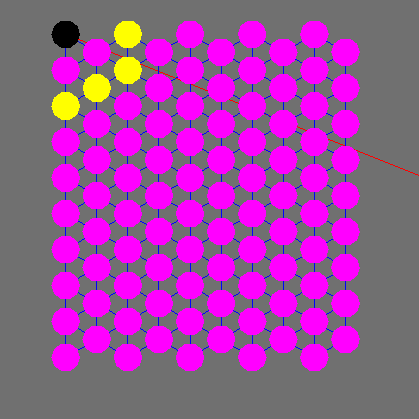
\includegraphics[width=2.5cm]{Images/front_1.png}
      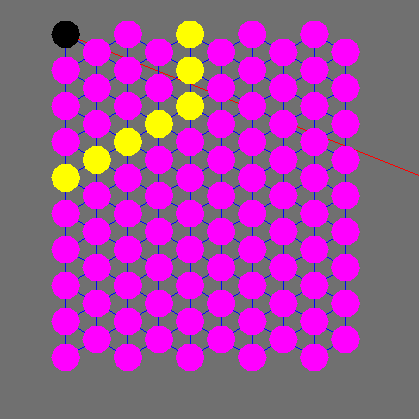
\includegraphics[width=2.5cm]{Images/front_2.png}
      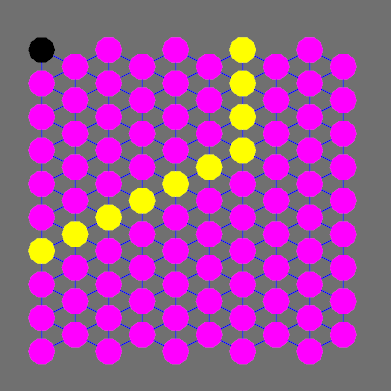
\includegraphics[width=2.5cm]{Images/front_3.png}
    \end{center}
    \begin{center}
      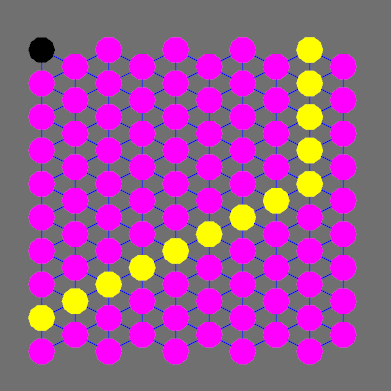
\includegraphics[width=2.5cm]{Images/front_4.png}
      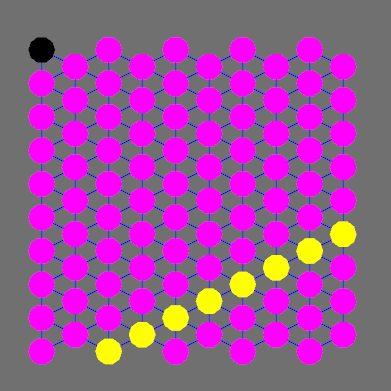
\includegraphics[width=2.5cm]{Images/front_5.png}
      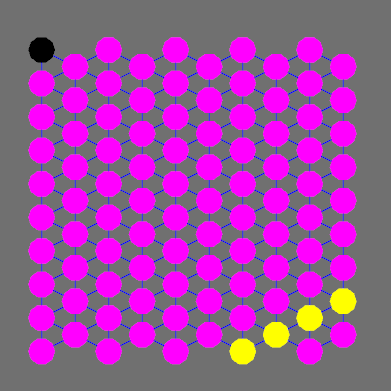
\includegraphics[width=2.5cm]{Images/front_6.png}
    \end{center}

    \caption{Bleu : liens entre cellules, Violet : cellules inactive, Noir : cellule de collision, Jaune : cellules appartenant au front.}
  \end{figure}
\end{frame}

\begin{frame}
  Utilisation d'un calque pour chaque cellule en collision. Fusion des calques avant le déplacement des cellules.
  \begin{figure}
    \begin{center}
      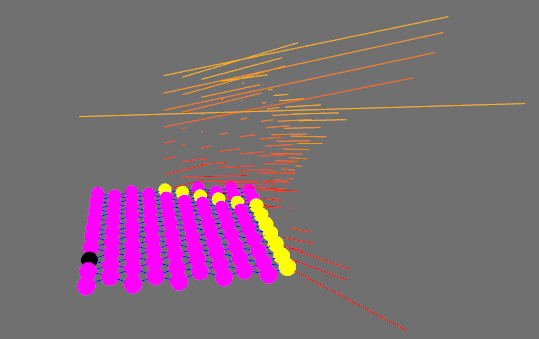
\includegraphics[width=6cm]{Images/layer.png}
    \end{center}
    \caption{Du rouge vers le jaune les différentes vélocités par cellules et par collisions.}
  \end{figure}
\end{frame}


\section{Les interactions entre cellules}
\subsection{Loi du centre instantané de rotation}
\begin{frame}
  \begin{multicols}{2}
    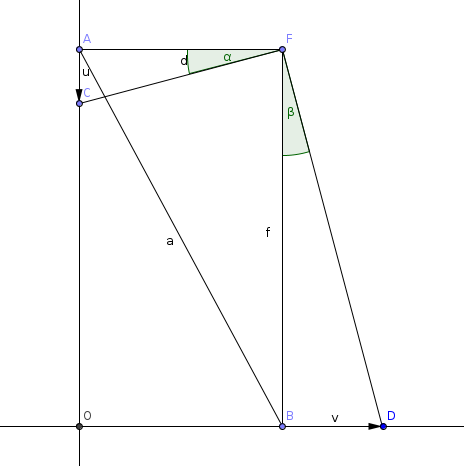
\includegraphics[width=5cm]{Images/geogebra_1.png}
    \vfill
    \columnbreak
    $\overrightarrow{u} = $ vélocité verticale \smallbreak
    $\overrightarrow{v} = $ vélocité horizontale \smallbreak
    $\alpha = \beta = $ rotation autour de F \smallbreak
    $||\overrightarrow{u}|| = \alpha \times d$ \smallbreak
    $||\overrightarrow{v}|| = \alpha \times f$ \smallbreak
    $\alpha = \frac{||\overrightarrow{u}||}{d}$ \smallbreak
  \end{multicols}
\end{frame}

\begin{frame}
  \begin{multicols}{2}
    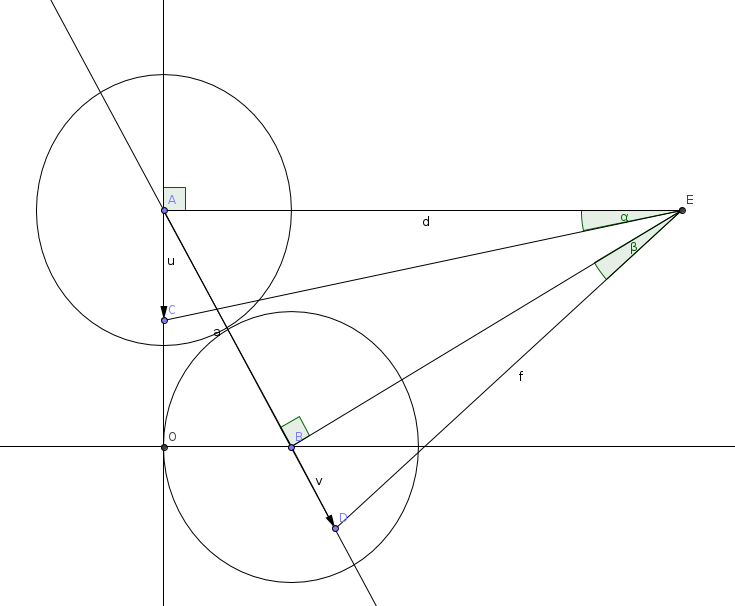
\includegraphics[width=6cm]{Images/geogebra_2.png}
    \vfill
    \columnbreak
    Si $(\overrightarrow{v}, \overrightarrow{u}) = 0$ \smallbreak
    $\overrightarrow{v} = \overrightarrow{u}$ \smallbreak
    $d = f = \infty$ \smallbreak
    Si $(\overrightarrow{u}, \overrightarrow{v}) = \frac{\pi}{2}$ \smallbreak
    $f = 0$ \smallbreak
    $\overrightarrow{v} = \overrightarrow{0}$
  \end{multicols}
\end{frame}

\begin{frame}
  \begin{figure}
    \begin{center}
      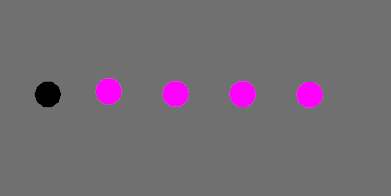
\includegraphics[width=3.5cm]{Images/cir_1.png}
      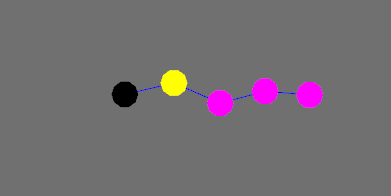
\includegraphics[width=3.5cm]{Images/cir_2.png}
      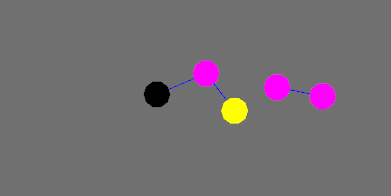
\includegraphics[width=3.5cm]{Images/cir_3.png}
    \end{center}
    \begin{center}
      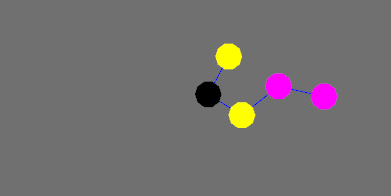
\includegraphics[width=3.5cm]{Images/cir_4.png}
      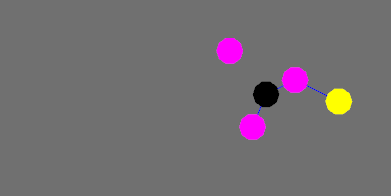
\includegraphics[width=3.5cm]{Images/cir_5.png}
      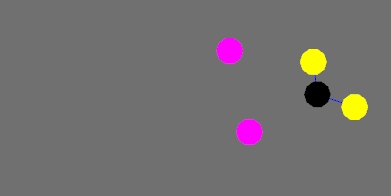
\includegraphics[width=3.5cm]{Images/cir_6.png}
    \end{center}
    \caption{6 échantillons de compressions avec le CIR.}
  \end{figure}
\end{frame}



\subsection{La loi de Hooke et le module de Young}
\begin{frame}
  \begin{center}
    $\sigma = E \times \varepsilon$
  \end{center}
  $\sigma = $ La force appliqué sur le matériau (en Pa). $E = $ Le module de Young pour le matériau étudié (en Pa). $\varepsilon = $ Coefficient de déformation (en $\%$). \smallbreak
  Module de Young :
  \begin{itemize}
    \item Granite : 60 GPa ;
    \item Calcaire : 20 à 70 GPa.
  \end{itemize}
  \smallbreak
  \begin{center}
    $\varepsilon = \frac{x_{max}}{\sqrt{x}}$
  \end{center}
  $x_{max} = $ La distance à respecter entre deux cellules. $x = $ La distance entre les deux cellules. \smallbreak
  \begin{center}
    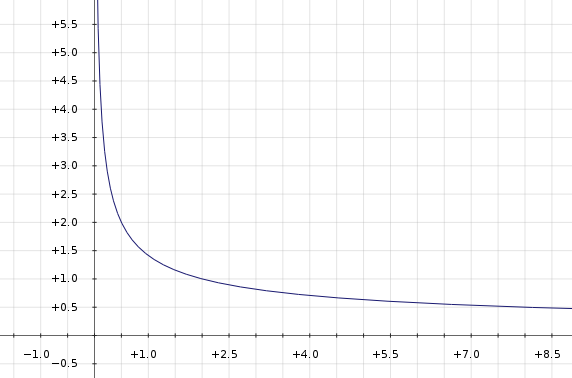
\includegraphics[width=3cm]{Images/compression_kmplot.png}
  \end{center}
\end{frame}

\begin{frame}
  \begin{figure}
    \begin{center}
      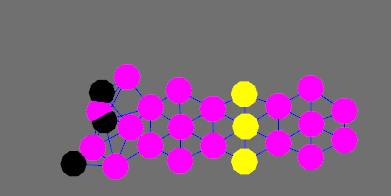
\includegraphics[width=6cm]{Images/no_compression.png}
      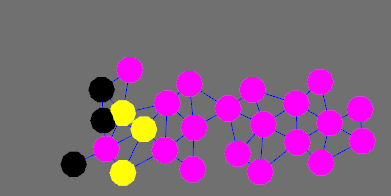
\includegraphics[width=6cm]{Images/compression.png}
    \end{center}
    \caption{A gauche simulation sans compression et à droite avec compression.}
  \end{figure}
\end{frame}


\subsection{La loi de Coulomb}
\begin{frame}
  \begin{figure}
    \begin{center}
      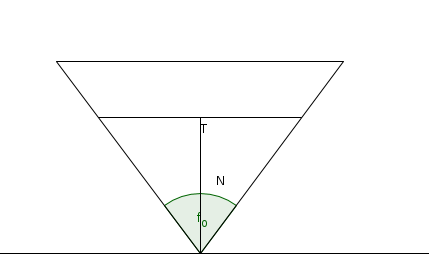
\includegraphics[width=5cm]{Images/friction.png}
    \end{center}
    \caption{Le cône représentant la force maximale possible avant un glissement.}
  \end{figure}
  \begin{center}
    $T_0 = f_0 \times N$
  \end{center}
  Si $T > T_0$ : glissement. Sinon friction. \smallbreak
  Où $T = $ force tangentielle appliquée à la cellule, $N = $ la pression entre les cellules et $f_0 = $ le coefficient d'adhérence.
\end{frame}






\end{document}
